\subsubsection{Presentation}
Decision Trees are a supervised learning model.\\
Decision Trees work by constructing a tree of features and value ranges, then traversing this tree to reach the classes at the leaf, they try to keep this tree balanced, but it isn't always.\\
The main hyperparameter to tune is the depth of this tree.

\subsubsection{Defining Parameters}
The data for training and validating is already defined by the Data Preparation step (80\% train, 20\% validation).\\
Representative parameter for this model is \emph{max\_depth}: The maximum depth of the constructed decision tree, the deeper the tree, the more likely it is to overfit the data.\\
Applying the algorithm with default \emph{max\_depth} (None) resulted in 94\% accuracy.\\
Tuning \emph{max\_depth} with GridSearch algorithm over a range of values resulted in highest accuracy achieved at \emph{max\_depth}=13.\\
Applying the algorithm again over that same range, but validating using the test dataset shows very similar results, as shown in the plot below.
\begin{center}
    \captionsetup{type=figure}
    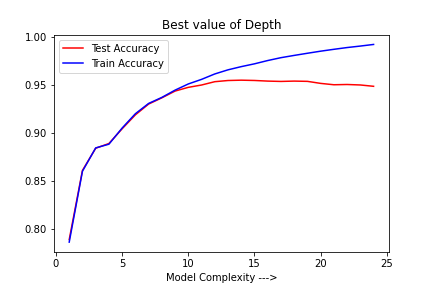
\includegraphics[width=250px]{DT_complexity.png}
    \captionof{figure}{Complexity Curve: \emph{max\_depth} value for DecisionTreeClassifier}
\end{center}
The model starts to overfit the training data after \emph{max\_depth}=13

\subsubsection{Model Evaluation}

Using the parameter \emph{max\_depth}=13, we plot the learning curve showing test and validation scores

\begin{center}
    \captionsetup{type=figure}
    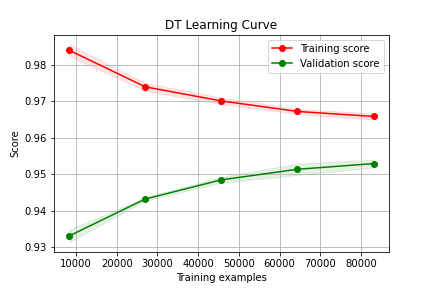
\includegraphics[width=250px]{learning_curve_DT.png}
    \captionof{figure}{Learning Curve for DT}
\end{center}
Both the variance and bias are lowering as we use more training data. \\
Observing the learning curve we see that the results start to converge, increasing the size of the dataset may increase the accuracy.
